\documentclass[letterpaper]{article}

\usepackage[utf8]{inputenc}
\usepackage[T1]{fontenc}
\usepackage{amsmath}
\usepackage{amssymb}
\usepackage{fancyhdr}
\usepackage{graphicx}
\usepackage{lastpage}
\usepackage{hyperref}
\hypersetup{
    unicode=true,
    pdftitle={The \$t\^{o}kEx Algorithm: a continuous, order-book-free exchange mechanism between two fungible assets},
    pdfauthor={Maxime Tousignant and Milu (Smoothop)},
    pdfsubject={Defensive publication: the exchange algorithm of the t\^{o}k system},
    pdfkeywords={exchange algorithm, market mechanism, automated market maker, AMM, order book, continuous trading, market clearing, equilibrium price, currency exchange, TWAP, tok, Smoothop}
}
\usepackage{tabularx}
\usepackage{geometry}
\usepackage{algorithmic}
\usepackage[safe]{tipa}

% Page size and spacing
\geometry{letterpaper,left=1in, right=1in, top=1in, bottom=1in}
\setlength{\parskip}{5pt}
\setlength{\parindent}{0pt}

% Header and footer
\pagestyle{fancy}
\fancyhead[L]{Smoothop}
\fancyhead[C]{Defensive Publication}
\fancyhead[R]{July 2026}
\fancyfoot[L]{}
\fancyfoot[C]{}
\fancyfoot[R]{page \thepage /\pageref*{LastPage}}

\newcommand{\priceAB}{\left[\alpha / \beta\right]}
\newcommand{\priceBA}{\left[\beta / \alpha\right]}
\newcommand{\tokEx}{\$t\^{o}kEx}

\DeclareMathOperator*{\argmax}{arg\,max}
\DeclareMathOperator*{\argmin}{arg\,min}

% ----------------------------------------------------------------------
\begin{document}\thispagestyle{plain}
% ----------------------------------------------------------------------

\begin{center}

\includegraphics[height=1in]{smoothop_logo.pdf}

\vspace{12pt}
{\LARGE \textbf{The \tokEx{} Algorithm}}

\vspace{6pt}
{\large A continuous, order-book-free exchange mechanism\\ between two fungible assets}

\vspace{12pt}
Maxime Tousignant\textsuperscript{1} \quad and \quad Milu\textsuperscript{1,2}

\vspace{4pt}
{\small \textsuperscript{1}\,Organisme de d\'eveloppement durable Smoothop, Montr\'eal, Canada\\
\textsuperscript{2}\,Anthropic (Milu is an AI agent built on Anthropic's Claude models)\\
Contact: \texttt{maxime.tousignant@smoothop.org}}

\vspace{6pt}
\textit{Original technical memorandum: January 2022.\\ Published as a defensive publication: July 2026.}
\end{center}

\subsection*{Defensive publication notice}
This document is made public in order to place the methods it describes in the prior art. Its publication is intended to preclude the grant of valid patent claims on these methods by any party. No exclusivity is sought by the publisher. This document is distributed under the Creative Commons Attribution 4.0 International license (CC BY 4.0). The \tokEx{} algorithm is part of the t\^{o}k system, an alternative economic system developed by Smoothop (\url{https://www.smoothop.org/}).

\subsection*{Name and pronunciation}
The name \tokEx{} juxtaposes the two currencies of the exchange (the dollar and the t\^{o}k), followed by ``Ex'' for exchange. It is pronounced \textipa{[stOkEks]}: the dollar sign is read as an ``S''.

\subsection*{Abstract}
The \tokEx{} is an algorithm for the continuous exchange of two fungible assets, A and B, without an order book and without counterparty matching. Each participant declares an estimate of the relative value of the two assets and a degree of certainty in that estimate. The degree of certainty is mapped to a weight through $w = \frac{1}{3}\tan\left(\pi\,\theta/200\,\%\right)$; geometrically, $\theta$ is the angle of the participant's response curve at its equilibrium point. Every participant exchanges continuously, at velocities given by a common trader function $f(x) = x^2 - 1/x$ of the ratio between the market price and the participant's estimate; both assets are treated symmetrically and all exchanges occur exactly at the market price. The market price is the unique positive price that simultaneously clears both assets; it has the closed form given in Eq.~\eqref{eqMarketPrice}. The whole market is provably indistinguishable from a single participant with an aggregate weight and degree of certainty. The state of the market is piecewise constant between events and is advanced exactly, event by event, by the two algorithms given below, with incremental $O(N \log N)$ updates. Mathematical proofs are provided in the annexes.

\textbf{Keywords:} exchange algorithm, market mechanism, automated market maker (AMM), order book, decentralized exchange, continuous trading, market clearing, equilibrium price, currency exchange, time-weighted execution (TWAP).

\subsection*{Relation to known mechanisms}
The \tokEx{} is an automated exchange mechanism, but it differs from the known families of market designs. Unlike the continuous double auction (the order book of stock and cryptocurrency exchanges), it involves no orders, no bids or asks, and no counterparty matching. Unlike the automated market makers (AMM) and constant-function market makers of decentralized exchanges (constant-product pools and their generalizations), it holds no liquidity pool and derives no price from reserves: the price is computed in closed form from the participants' declared estimates and degrees of certainty, and the participants trade with each other, continuously, exactly at that price. The continuous execution spreads each transaction over time, as time-weighted average price (TWAP) execution strategies do on traditional markets, but here the property belongs to the market itself: supply and demand clear exactly at every instant.

% ----------------------------------------------------------------------
\section{Notation}
% ----------------------------------------------------------------------

\begin{tabularx}{\textwidth}{rX}
 $\alpha$ & Symbol for asset A  \\
 $\beta$ & Symbol for asset B  \\
 $\priceAB$ & The value of 1 unit of $\beta$ priced in $\alpha$ \\
 $\priceBA$ & The value of 1 unit of $\alpha$ priced in $\beta$ (note: $\priceBA= \priceAB^{-1}$) \\
 $\dot{X}^\alpha$ & Exchange velocity of asset A (in $\alpha$ / unit of time): the contribution of the exchange to the rate of change of a wallet's balance $n^\alpha$, positive when the wallet receives asset A \\
 $\dot{X}^\beta$ & Exchange velocity of asset B (in $\beta$ / unit of time), with the same sign convention \\
 $n^\alpha$ & Amount in an account holding asset A (in $\alpha$)\\
 $n^\beta$ & Amount in an account holding asset B (in $\beta$)\\
 $?_i$ & quantity related to the $i$\textsuperscript{th} participant \\
 $?_\Omega$ & quantity related to the market
\end{tabularx}

% ----------------------------------------------------------------------
\section{Principles of the \tokEx{} Algorithm}
% ----------------------------------------------------------------------

The purpose of the algorithm is to set up a market between different participants in which two fungible assets, A and B, can be \textbf{continuously} exchanged according to each participant's estimate of the relative value of the two assets.

\textbf{Wallets.} Each participant holds a \emph{wallet}: one account per asset, with balances $n^\alpha$ and $n^\beta$. Individual balances evolve continuously through the exchanges of the \tokEx{}, and also through channels external to it: the participant's own deposits and withdrawals, and any intrinsic dynamics of the asset itself (a demurrage, for instance). The exchange in itself only moves amounts between wallets: it leaves the \emph{sums} $\sum_i n^\alpha_i$ and $\sum_i n^\beta_i$ unchanged.

The algorithm obeys eight fundamental principles, which fall into two classes: the \emph{fair-market principles} (1--4), which constrain the market itself, and the \emph{rational-trader principles} (5--8), which specify the behavior of the participants, a behavior implemented for all participants by the same function, called the \emph{trader function}.

\textbf{Fair-market principles} (the market is unbiased):
\begin{enumerate}
    \item \emph{Equilibrium and conservation.} The market price is the price at which supply meets demand: at any given time, whatever amount of an asset some participants sell must be bought by others, and vice versa,
    \begin{equation*}
        \sum_i \dot{X}_i^\alpha = \sum_i \dot{X}_i^\beta = 0\,.
    \end{equation*}
    Since $\dot{X}_i$ is precisely the contribution of the exchange to the balance $n_i$, the same equation is a conservation law: the exchange creates and destroys nothing, it only transfers existing amounts between the participants' wallets. Every other channel through which a balance can change (deposits, withdrawals, the intrinsic dynamics of the asset itself, such as a demurrage) is external to the \tokEx{} and accounted for separately.
    \item \emph{Exchange at market price.} At any given time there is a single market price, strictly positive and common to all participants, and every exchange takes place exactly at it:
    \begin{equation*}
        \priceAB_\Omega = -\,\frac{\dot{X}_i^\alpha}{\dot{X}_i^\beta} > 0 \quad \text{for every trading participant } i\,.
    \end{equation*}
    \item \emph{No bias between participants.} All exchange velocities are given by one common function of the participant's own inputs and of the market state, the same function for every participant:
    \begin{equation*}
        \dot{X}_i^\alpha = F\!\left(\priceAB_i,\ \theta_i\ ;\ \priceAB_\Omega\right) \quad \text{for all } i\,.
    \end{equation*}
    \item \emph{No bias between assets.} The defining equations are invariant under swapping the two assets:
    \begin{equation*}
        \alpha \leftrightarrow \beta \quad \left(\text{hence } \priceAB \leftrightarrow \priceBA\right).
    \end{equation*}
\end{enumerate}

\textbf{Rational-trader principles} (every participant trades rationally). Let $x_i := \priceAB_\Omega / \priceAB_i$ denote the ratio between the market price and the $i$\textsuperscript{th} participant's estimate:
\begin{enumerate}
    \setcounter{enumi}{4}
    \item \emph{Buy low.} When the market prices an asset below the participant's estimate, the participant is willing to buy that asset:
    \begin{equation*}
        x_i < 1 \;\Longrightarrow\; \dot{X}_i^\beta > 0 \ \left(\text{and } \dot{X}_i^\alpha < 0\right).
    \end{equation*}
    \item \emph{Sell high.} When the market prices it above the estimate, the participant is willing to sell it; at the estimate, they do not trade:
    \begin{equation*}
        x_i > 1 \;\Longrightarrow\; \dot{X}_i^\beta < 0 \ \left(\text{and } \dot{X}_i^\alpha > 0\right); \qquad x_i = 1 \;\Longrightarrow\; \dot{X}_i^\alpha = \dot{X}_i^\beta = 0\,.
    \end{equation*}
    \item \emph{Urgency grows with the gap.} The exchange velocity increases strictly with the distance between market price and estimate:
    \begin{equation*}
        \dot{X}_i^\alpha \ \text{is strictly increasing in } x_i\,,
    \end{equation*}
    so that $|\dot{X}_i^\alpha|$ grows as $x_i$ moves away from 1 in either direction.
    \item \emph{Urgency grows with certainty.} Velocities scale with a weight that increases strictly with the degree of certainty:
    \begin{equation*}
        \dot{X}_i \propto w(\theta_i)\,, \quad w \ \text{strictly increasing},\quad w(0) = 0
    \end{equation*}
    No conviction, no trade.
\end{enumerate}

These eight principles are the \emph{hypotheses} of the \tokEx{}: everything that follows is constructed to satisfy them. The trader function \eqref{eqTraderFunction} realizes principles 5--8, the symmetric velocity pair \eqref{eqExchangeSymmetry} realizes principles 2--4, and the market price \eqref{eqMarketPrice} realizes principle 1.

\clearpage

% ----------------------------------------------------------------------
\section{Core Equations of the \tokEx{} Algorithm}
% ----------------------------------------------------------------------

Exchanges on the \tokEx{} are continuous, instead of discrete in time like on traditional markets. For example, rather than buying 5 units of $\beta$ in exchange for 10~units of $\alpha$ at some instant~$t$ on a traditional market (which implies a market price of 2~$\alpha$ per~$\beta$), the same exchange on the \tokEx{} could happen by continuously buying units of~$\beta$ (at the market price of 2~$\alpha$ per~$\beta$) with a velocity of 1~$\beta$ per hour for 5 hours.

On the participant level, the advantage of a continuous exchange is that, by spreading their transaction over a longer period of time, they reduce the risk of making their transaction at a bad time. As we will show, the \tokEx{} allows the participant to automatically either buy or sell more (i.e. at a higher velocity) when the market price is more advantageous for them.

At the market level, the advantage of a continuous exchange is that the market price would potentially be more stable since every participant is automatically reacting to any change in the market price by increasing or decreasing their exchange velocities.

\subsection{Participant's exchange velocities}
% ----------------------------------------------------------------------

Every participant in the \tokEx{} has their exchange velocities determined by the same function. In that sense, the \tokEx{} is not biased towards a participant or another and therefore fulfills principle number~3 mentioned earlier.

This function requires two inputs from the participant:

\begin{tabularx}{\textwidth}{rX}
 $[\alpha/\beta]_i$ & $i$\textsuperscript{th} participant's estimate of the value of 1~unit of~$\beta$ priced in~$\alpha$ \\
$\theta_i$ & $i$\textsuperscript{th} participant's degree of certainty (0-100\%) in their estimate of the relative value of the two assets.
\end{tabularx}

The function controlling the participant's exchange velocities in the \tokEx{} takes the following form:
\begin{align}
\dot{X}^\alpha_i &= w\!\left(\theta_i\right)\, f\!\left(\frac{\hspace{2pt}\priceAB_\Omega}{\priceAB_i} \right) \, \dot{R} \nonumber \, , \\
\dot{X}^\beta_i &=  w\!\left(\theta_i\right)\, f\!\left(\frac{\hspace{2pt}\priceBA_\Omega}{\priceBA_i} \right) \, \dot{R} \priceBA_i \,,
\label{eqExchangeSymmetry}
\end{align}
where $\dot{R}$ is the reference exchange velocity (in $\alpha$ / unit of time) for this particular exchange. The algorithm requires that a reference exchange velocity, constant and common to all participants, be defined for one of the two assets. For example, in a market where gold is exchanged for dollars, the reference exchange velocity could be set to 1~dollar per hour or 1~ounce of gold per day or whatever reference velocity makes sense in the context of that particular market.

By convention, the reference exchange velocity $\dot{R}$ is defined in terms of asset A. The corresponding reference exchange velocity for asset B is $\dot{R} \priceBA_i$ in the eyes of the $i$\textsuperscript{th} participant. Apart from this difference, the two equations in \eqref{eqExchangeSymmetry} are perfectly symmetric in the sense that they are the same except that $\alpha$ is swapped with $\beta$. This property ensures that the market is not biased towards one asset or the other. Therefore, the form of the function controlling a participant's exchange velocities satisfies principle number~4.

Next, we need to specify the functions~$w$ and~$f$ that compose the exchange velocities function. Let us first define the \emph{trader function}~$f$. This function describes the general behavior of a participant depending on the ratio between the market price $\priceAB_\Omega$ and their estimate of the value of $\priceAB$. This general behavior follows principles number~5, 6 and~7. The \tokEx{} satisfies these principles by defining the trader function, for any price ratio $x > 0$, as
\begin{equation}
    f(x) = x^2 - \frac{1}{x}\,. \label{eqTraderFunction}
\end{equation}
This choice is principled but not arbitrary. As shown in Annex~\ref{secTraderFamily}, principles 2 and 4 by themselves force two structural properties of any admissible trader function: the functional equation $f(1/x) = -f(x)/x$, and hence $f(1) = 0$ (no trade at one's own estimate). The functions compatible with all eight principles and with a closed-form market price form a one-parameter family, of which \eqref{eqTraderFunction} is the minimal member with unbounded urgency on both the buying and the selling side; the whole family is described in Annex~\ref{secTraderFamily} and is part of the present disclosure.

Each participant evaluates it at the ratio between the market price and their own estimate:
\begin{align}
f_i^\alpha &:= f\!\left(\frac{\hspace{2pt}\priceAB_\Omega}{\priceAB_i} \right) =  \left( \frac{\hspace{2pt}\priceAB_\Omega}{\priceAB_i}\right)^2 - \frac{\priceAB_i}{\hspace{2pt}\priceAB_\Omega} \, , \nonumber \\
f_i^\beta &:= f\!\left(\frac{\hspace{2pt}\priceBA_\Omega}{\priceBA_i} \right) = \left( \frac{\hspace{2pt}\priceBA_\Omega}{\priceBA_i}\right)^2 - \frac{\priceBA_i}{\hspace{2pt}\priceBA_\Omega} \, .
\label{eqFunctionX}
\end{align}

Second, we define the function $w$ that serves as a weighting factor for each participant in the \tokEx{}. It maps a participant's degree of certainty $[0, 100)\,\%$ onto $[0,+\infty)$, such that
\begin{equation}
    w_i := w\left(\theta_i\right) = \frac{1}{3}\tan \left( \frac{\pi \,\theta_i}{200\%}\right)\,. \label{eqFunctionW}
\end{equation}
The function $w$ is consistent with principle number 8 since it scales the participant's exchange velocities according to their degree of certainty (we show in Annex \ref{secProofDegree} that $\theta_i$ can be interpreted as a geometrical angle in the right context).

Thus, the exact expressions for the exchange velocities of the $i$\textsuperscript{th} participant are
\begin{align}
    \dot{X}^\alpha_i &= w_i \left( \left( \frac{\hspace{2pt}\priceAB_\Omega}{\priceAB_i}\right)^2 - \frac{\priceAB_i}{\hspace{2pt}\priceAB_\Omega} \right) \dot{R}\,, \nonumber\\
    \dot{X}^\beta_i &= w_i \left( \left( \frac{\hspace{2pt}\priceBA_\Omega}{\priceBA_i}\right)^2 - \frac{\priceBA_i}{\hspace{2pt}\priceBA_\Omega} \right) \dot{R} \priceBA_i\,. \label{eqExchangeVelocities}
\end{align}
In Fig.~\ref{figExchangeSymmetry}, we can see that indeed, the expressions in \eqref{eqExchangeVelocities} are symmetric (unbiased toward one asset or the other) and that they allow each participant to automatically ``buy low and sell high" according to their estimate of the relative value of assets~A and~B.

\begin{figure}[b!]
\centering
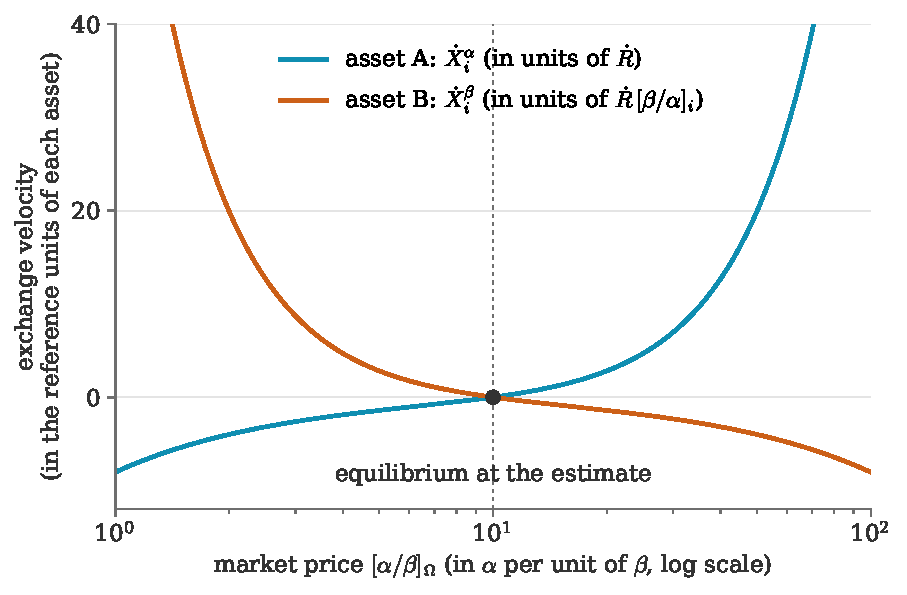
\includegraphics[width=0.75\textwidth]{stok-market_symmetry.pdf}
\caption{$i$\textsuperscript{th} participant's exchange velocities with $\priceAB_i = 10$~$\alpha$ per~$\beta$, and $\theta_i= 75 \%$}
\label{figExchangeSymmetry}
\end{figure}

In Annex \ref{secProofExchangeAtMarketPrice}, we prove that the expressions in \eqref{eqExchangeVelocities} are consistent with principle number~2, which states that every participant buys and sells at market price. Formally, this means that
\begin{equation}\label{eqExchangeAtMarketPrice}
    \left[\alpha/\beta\right]_\Omega = - \frac{\dot{X}^\alpha_i}{\dot{X}^\beta_i} \,.
\end{equation}
Indeed, if a participant is buying asset A and paying with asset B, the two exchange velocities must be of opposite sign and the proportionality constant between the two is the market price. In Sec.~\ref{secMarketPrice}, we will determine the expression to compute the market price $\priceAB_\Omega$.

\subsection{Time it takes to empty a participant's account}
% ----------------------------------------------------------------------

With the participant's exchange velocities, we can predict when their account balance is going to reach zero. The account that will eventually be empty is the account holding the asset that the participant is selling (i.e. the account holding the asset for which $\dot{X}_i < 0$). The general principle is this: as long as the state of the market is constant, the balance obeys $\dot{n}_i = \dot{X}_i + (\text{intrinsic dynamics of the asset})$, and $\Delta t_i$ is the first time at which $n_i(t)$ reaches zero. A participant who is not selling ($\dot{X}_i \geq 0$) never empties an account: $\Delta t_i = +\infty$.

For a \emph{regular} asset (no intrinsic dynamics), the balance decreases linearly and
\begin{equation}\label{eqDeltaT}
    \Delta t_i = - \frac{n_i}{\dot{X}_i} \,.
\end{equation}

For an asset with a continuous exponential demurrage at rate $k$ (such as the t\^{o}k of the reference implementation), the balance obeys $\dot{n}_i = \dot{X}_i - k\, n_i$, whose solution reaches zero after
\begin{equation}\label{eqDeltaTDemurrage}
    \Delta t_i = \frac{1}{k} \ln\!\left(1 - \frac{k\, n_i}{\dot{X}_i}\right),
\end{equation}
which is shorter than \eqref{eqDeltaT} (the demurrage helps empty the account) and reduces to it as $k \to 0$. Since \eqref{eqDeltaTDemurrage} is a strictly increasing function of the linear estimate \eqref{eqDeltaT}, the transformation commutes with the minimum over participants taken by the outer algorithm: an implementation only needs to track \eqref{eqDeltaT} for every account, and to apply the logarithm once, to the minimum of the accounts sharing the same demurrage rate. The reference implementation does exactly this for the t\^{o}k side of the market, in the numerically stable $\operatorname{log1p}$ form.

\subsection{Market price}\label{secMarketPrice}
% ----------------------------------------------------------------------

As stated in principle number 1, the market price is the relative asset value that leads to an equilibrium between supply and demand. Formally, this means that the market price must satisfy
\begin{equation}
    \sum_i \dot{X}_i^\alpha = \sum_i \dot{X}_i^\beta = 0 \,. \label{eqEquilibrium}
\end{equation}
Indeed, at any given time and for both assets, the total amount being sold by some participants must be bought by some others: the \tokEx{} creates and destroys nothing, it only transfers.

Since the behavior of each participant is set in a rational way by \eqref{eqExchangeVelocities} and entirely defined by their two inputs $\priceAB_i$ and $\theta_i$, we find (see proof in Annex \ref{secProofMarketprice}) that the expression for the market price is
\begin{equation}
    \priceAB_\Omega = \left( \frac{\displaystyle \sum_i w_i \priceAB_i}{\displaystyle \sum_i w_i \priceBA_i^2}\right)^{1/3}\,. \label{eqMarketPrice}
\end{equation}
In this expression, the sum over the participants only includes those who are actually able to trade (i.e. they have the asset they wish to sell).

Let us note that this equilibrium price is \emph{unique}: by principle 7, each participant's exchange velocity is strictly increasing in the market price, hence so is the net flow $\sum_i \dot{X}_i^\alpha$, so it can vanish at only one strictly positive price, the one given by \eqref{eqMarketPrice}. The precise conditions and the proof are given in Annex~\ref{secProofUniqueness}.

\clearpage

% ----------------------------------------------------------------------
\section{Implementation of the \tokEx{} Algorithm}
% ----------------------------------------------------------------------

The equations of the \tokEx{} that were developed in the previous section are valid as long as both inputs from all participants remain constant and as long as each participant has a positive balance in the account holding the asset they are selling. Of course, at some point in time, these conditions are bound to change. Therefore, the \tokEx{} operates in steps during which the state of the market remains constant (i.e. constant market price and constant exchange velocities).

In general, we know the balance of every account at $t_0$ and we want to know their balance at $t_1$, when a participant requests an action. The actions available to the participant are:
\begin{enumerate}
    \item check the market price,
    \item check their account balance,
    \item deposit/withdraw an amount,
    \item change their estimate or degree of certainty.
\end{enumerate}

Between $t_0$ and $t_1$, both inputs from all participants are constant. However, we must automatically handle the cases when one of the participants runs out of the asset they are selling between $t_0$ and $t_1$. Each time this happens, the state of the market must be updated.

Thus, the \tokEx{} is implemented in two parts. First we describe the inner algorithm responsible for outputting the current state of the market. Second we describe the outer algorithm that performs the time stepping to get from $t_0$ to $t_1$. This process is illustrated in Fig.~\ref{figMarketSteps}.

\begin{figure}[b!]
\centering
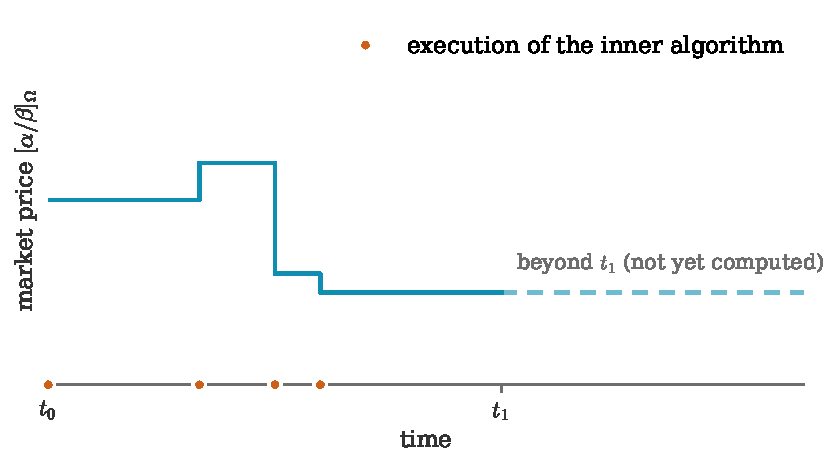
\includegraphics[width=0.75\textwidth]{stok-market_steps.pdf}
\caption{Process by which the state of the \tokEx{} is updated between $t_0$ and $t_1$.}
\label{figMarketSteps}
\end{figure}
\clearpage

\subsection{Inner \tokEx{} Algorithm}
% ----------------------------------------------------------------------

The purpose of the inner algorithm is to return the market price and participants' exchange velocities at the current time $t$. The inner algorithm takes into account that some participants might have run out of the asset they wish to sell. These participants must therefore be excluded from the market since their estimate is irrelevant. By excluded from the market, we mean that both their exchange velocities are zero and that their input parameters are not taken into account for the computation of the market price.

When a participant runs out of the asset they are selling, they are automatically excluded from the market. On the other hand, when the excluded participants are in a situation where they can participate again, they are also automatically reintegrated in the market.

\subsubsection{Inputs}
Each participant in the market must provide the following information:

\begin{tabularx}{\textwidth}{rX}
 $[\alpha/\beta]_i$ & $i$\textsuperscript{th} participant's estimate of the value of 1 unit of $\beta$ priced in $\alpha$ \\
$\theta_i$ & $i$\textsuperscript{th} participant's degree of certainty (0-100\%) in their estimate of the relative value of the two assets.
\end{tabularx}

In addition, we must provide to the algorithm the balance for both accounts of every participant at the current time $t$:

\begin{tabularx}{\textwidth}{rX}
 $n_i^\alpha$ & $i$\textsuperscript{th} participant's balance of asset A (in $\alpha$) \\
$n_i^\beta$ & $i$\textsuperscript{th} participant's balance of asset B (in $\beta$)
\end{tabularx}

\subsubsection{Outputs}
From the above inputs, the algorithm calculates and returns the following information:

\begin{tabularx}{\textwidth}{rX}
 $[\alpha/\beta]_\Omega$ & The market value of 1 unit of $\beta$ priced in $\alpha$ \\
$\dot{X}^\alpha_i$ & the $i$\textsuperscript{th} participant's exchange velocity of asset A (in $\alpha$ per unit of time)\\
$\dot{X}^\beta_i$ & the $i$\textsuperscript{th} participant's exchange velocity of asset B (in $\beta$ per unit of time) \\
$\Delta t_i$ & the amount of time after which the $i$\textsuperscript{th} participant runs out of the asset they are selling
\end{tabularx}

\subsubsection{Plain description of the inner \tokEx{} algorithm}
\begin{itemize}
    \item Exclude every participant that has at least one empty account from the market and add them to a checklist. (lines 3-10)
    \item Compute the market price using \eqref{eqMarketPrice}. (line 11)
    \item For each participant that has been excluded, check if they have a positive balance in the account holding the asset they wish to sell. If so, reintegrate them in the market and compute the new market price using \eqref{eqMarketPrice}. Once a participant has been checked, remove them from the checklist. Repeat this process until no participant is left on the checklist. Since reintegrating a participant in the market changes the market price, we have to be careful with the order in which we cross off the participants from the checklist. To ensure that this process is done properly, it can be shown that we must always check the participant whose value estimate is the ``furthest" away from the market price, our metric for the distance being $|f_i^\alpha|$, computed using \eqref{eqFunctionX}. To find that participant efficiently, the checklist is first \emph{sorted} by estimate: for any given price, since $f$ is monotone in the estimate, the largest $|f_i^\alpha|$ is always attained at one of the two ends of the sorted checklist, so each step examines two participants only, and each reintegration updates the market price in $O(1)$: the participant's terms are added to the two market sums of \eqref{eqMarketPrice} and the price is recomputed from them (the same incremental bookkeeping as the market update of Sec.~\ref{secMarketUpdate}). (lines 12-21)
    \item For each participant, compute their exchange velocities, using \eqref{eqExchangeVelocities}, and the time it will take to empty the account for the asset they are selling, using \eqref{eqDeltaT}. (lines 22-36)
\end{itemize}
\clearpage

\subsubsection{Pseudocode for the inner \tokEx{} algorithm}
\begin{algorithmic}[1]
    \STATE \textbf{given} the account balance $n_i^\alpha$ and $n_i^\beta$ for every participant
    \STATE \textbf{given} the inputs $\priceAB_i$ and $\theta_i$ for every participant
    \FORALL{participants}
        \IF{$n_i^\alpha = 0$ \OR $n_i^\beta = 0$}
            \STATE exclude $i$\textsuperscript{th} participant from the market
            \STATE add $i$\textsuperscript{th} participant to checklist
        \ELSE
            \STATE include $i$\textsuperscript{th} participant in the market
        \ENDIF
    \ENDFOR
    \STATE compute $\priceAB_\Omega$
    \STATE sort the checklist by increasing estimate $\priceAB_i$
    \WHILE{checklist is not empty}
        \STATE compute $f^\alpha$ at both ends of the checklist
        \STATE $i^{\ast} \gets$ the end with the largest $|f^\alpha|$
        \IF{($f_{i^{\ast}}^\alpha \geq 0$ \AND $n_{i^{\ast}}^\beta > 0$) \OR ($f_{i^{\ast}}^\alpha \leq 0$ \AND $n_{i^{\ast}}^\alpha > 0$)}
            \STATE include $i^{\ast}$\textsuperscript{th} participant in the market
            \STATE update $\priceAB_\Omega$ incrementally
        \ENDIF
        \STATE remove $i^{\ast}$\textsuperscript{th} participant from checklist
    \ENDWHILE
    \FORALL{participants}
        \IF{$i$\textsuperscript{th} participant is included in the market}
            \STATE compute $\dot{X}_i^\alpha$ and $\dot{X}_i^\beta$
        \ELSE
            \STATE $\dot{X}_i^\alpha \gets 0$ and $\dot{X}_i^\beta \gets 0$
        \ENDIF
        \IF{$\dot{X}_i^\alpha < 0$}
            \STATE $\Delta t_i \gets - n_i^\alpha / \dot{X}_i^\alpha$
        \ELSIF{$\dot{X}_i^\beta < 0$}
            \STATE $\Delta t_i \gets - n_i^\beta / \dot{X}_i^\beta$
        \ELSE
            \STATE $\Delta t_i \gets +\infty$
        \ENDIF
    \ENDFOR
    \RETURN $\priceAB_\Omega$, $\dot{X}_i^\alpha$, $\dot{X}_i^\beta$ and $\Delta t_i$
\end{algorithmic}
\clearpage

\textbf{Complexity.} The exclusion pass, the from-scratch market price and the final velocity computation are all $O(N)$; the checklist sort is $O(N \log N)$; each reintegration step costs $O(1)$ thanks to the incremental update of the two market sums. The inner \tokEx{} algorithm therefore runs in $O(N \log N)$ overall.

\subsection{Outer \tokEx{} Algorithm}
% ----------------------------------------------------------------------

The outer algorithm performs the necessary time steps to get from $t_0$ to $t_1$. If a participant runs out of the asset they are selling during that time interval, the outer algorithm steps up to that instant to update the state of the market. This process repeats until $t_1$ is reached.

\subsubsection{Inputs}

\begin{tabularx}{\textwidth}{rX}
 $t_0$ & Initial time \\
$t_1$ & Final time
\end{tabularx}

Each participant in the market must provide the following information:

\begin{tabularx}{\textwidth}{rX}
 $[\alpha/\beta]_i$ & $i$\textsuperscript{th} participant's estimate of the value of 1 unit of $\beta$ priced in $\alpha$ \\
$\theta_i$ & $i$\textsuperscript{th} participant's degree of certainty (0-100\%) in their estimate of the relative value of the two assets.
\end{tabularx}

In addition, we must provide to the algorithm the balance for both accounts of every participant at the initial time $t_0$:

\begin{tabularx}{\textwidth}{rX}
 $n_i^\alpha$ & $i$\textsuperscript{th} participant's balance of asset A (in $\alpha$) \\
$n_i^\beta$ & $i$\textsuperscript{th} participant's balance of asset B (in $\beta$)
\end{tabularx}

\subsubsection{Outputs}
From the above inputs, the algorithm calculates and returns the market price and the balance for both accounts of every participant at $t_1$:

\begin{tabularx}{\textwidth}{rX}
 $[\alpha/\beta]_\Omega$ & The market value of 1 unit of $\beta$ priced in $\alpha$ \\
 $n_i^\alpha$ & $i$\textsuperscript{th} participant's balance of asset A (in $\alpha$) \\
$n_i^\beta$ & $i$\textsuperscript{th} participant's balance of asset B (in $\beta$)
\end{tabularx}

\subsubsection{Pseudocode for the outer \tokEx{} algorithm}

\begin{algorithmic}[1]
    \STATE \textbf{given} an initial time $t_0$
    \STATE \textbf{given} a final time $t_1$
    \STATE \textbf{given} the account balances $n_i^\alpha$ and $n_i^\beta$ for every participant (at $t_0$)
    \STATE \textbf{given} the inputs $\priceAB_i$ and $\theta_i$ for every participant (constant between $t_0$ and $t_1$)
    \STATE $t \gets t_0$
    \STATE \textbf{execute} inner \tokEx{} algorithm
    \STATE $\Delta t \gets \min_i \Delta t_i$
    \WHILE{$t_1 - t \geq \Delta t$}
        \FORALL{participants}
            \STATE $n_i^\alpha \gets n_i^\alpha + \dot{X}_i^\alpha \Delta t$
            \STATE $n_i^\beta \gets n_i^\beta + \dot{X}_i^\beta \Delta t$
        \ENDFOR
        \STATE $t \gets t + \Delta t$
        \STATE \textbf{execute} inner \tokEx{} algorithm
        \STATE $\Delta t \gets \min_i \Delta t_i$
    \ENDWHILE
    \STATE $\Delta t \gets t_1 - t$
    \FORALL{participants}
        \STATE $n_i^\alpha \gets n_i^\alpha + \dot{X}_i^\alpha \Delta t$
        \STATE $n_i^\beta \gets n_i^\beta + \dot{X}_i^\beta \Delta t$
    \ENDFOR
    \RETURN $n_i^\alpha$, $n_i^\beta$ and $\priceAB_\Omega$ (at $t_1$)
\end{algorithmic}

The pseudocode above is written for regular assets: the balance-update lines $n_i \gets n_i + \dot{X}_i\, \Delta t$ integrate $\dot{n}_i = \dot{X}_i$ exactly. For an asset with intrinsic dynamics, these lines and the $\Delta t_i$ of the inner algorithm are replaced by the closed-form solution of the corresponding balance equation (for a demurrage, the exponential behind \eqref{eqDeltaTDemurrage}); the event-driven structure of both algorithms is unchanged, and the stepping remains exact.

\subsection{Numerical evaluation of the trader function}\label{secNumTraderFunction}
% ----------------------------------------------------------------------

The typical operating point of the \tokEx{} is $x \approx 1$: participants' estimates hover around the market price. Precisely there, the defining expression $f(x) = x^2 - 1/x$ suffers \emph{catastrophic cancellation} in floating-point arithmetic: both terms are close to 1, and their subtraction erases up to half of the significand. Measured against exact rational arithmetic (IEEE-754 double precision), the relative error of the standard form reaches $4 \times 10^{-2}$ at $x = 1 - 10^{-15}$, and the algebraically equivalent form $(x^3-1)/x$ still errs by $\sim 10^{-9}$ at $x = 1 \pm 10^{-9}$.

The remedy is the \emph{shifted form}. Let $y = x - 1$; for $x \in [1/2,\ 2]$ this subtraction is exact in floating point (Sterbenz's lemma), and $x^3 - 1 = y^3 + 3y^2 + 3y$, so that
\begin{equation}
    f(x) = \frac{y\left(y^2 + 3y + 3\right)}{x}\,, \qquad y = x - 1\,. \label{eqShiftedForm}
\end{equation}
The numerator tracks the small deviation $y$ directly, without cancellation, and the denominator must be the \emph{input} $x$ itself: recomputing it as $y + 1$ reintroduces a relative error that grows toward the ends of the domain, up to $\sim 10^{-5}$ at $x = 10^{-12}$. The expression is branchless and constant-time (a straight line of fused multiply-adds, no conditional jumps), and its measured relative error stays below $6 \times 10^{-16}$ (machine precision) over the whole admissible domain of the ratio, $[10^{-12},\ 10^{12}]$. This domain is wider than the price bounds of the reference implementation: estimates are bounded to $[10^{-6},\ 10^{6}]$ and the market price always lies between the smallest and the largest estimate (see the corollary in Annex~\ref{secProofUniqueness}), so the \emph{ratio} of the two spans up to twelve decades on each side of 1.

\subsection{Reference implementation in the t\^{o}k system}
% ----------------------------------------------------------------------

In the t\^{o}k system, the \tokEx{} is instantiated with $\alpha$ = the t\^{o}k (a universal-income-based currency with continuous exponential demurrage) and $\beta$ = a foreign currency (CAD, EUR, \ldots), with one market per foreign currency. The reference implementation uses the following parameters: the reference exchange velocity $\dot{R}$ is set to the universal income rate of the t\^{o}k system (1~t\^{o}k per 15~days); estimates are bounded to $10^{-6} \leq \priceAB_i \leq 10^{6}$; degrees of certainty are discretized with a step of $10^{-4}\,\%$ and capped at $99.9999\,\%$; the default market price of an empty market is 1. Each participant holds a dedicated pair of market accounts (one per asset) with the same owner, and solvency is handled by per-asset tolerance thresholds. Market sums are computed with compensated (Kahan) summation in extended precision, updates are incremental, in $O(N \log N)$ overall (the solvency checklist is processed in sorted order of the estimates, the participant farthest from the market price always lying at one of its two ends), and the trader function is evaluated in the shifted form \eqref{eqShiftedForm} of Sec.~\ref{secNumTraderFunction}. The demurrage of the t\^{o}k acts on the t\^{o}k balances independently of the exchange velocities, consistently with principle 1: the \tokEx{} itself only transfers.

\clearpage

% ----------------------------------------------------------------------
\section{Market analysis}
% ----------------------------------------------------------------------

In this section we build some additional mathematical tools that may provide helpful insights into a market that uses the \tokEx{} algorithm. Among other things, the information about the market provided by these tools may help some participants to make their estimation.

\subsection{Market behavior}\label{secMarketBehavior}
% ----------------------------------------------------------------------

We define the market behavior as the sum of the behavior of all its participants, such that
\begin{equation}
    \dot{X}_\Omega^\alpha = \sum_i w_i \left( \left( \frac{\priceAB_z}{\priceAB_i}\right)^2 - \frac{\priceAB_i}{\priceAB_z} \right) \dot{R} \,, \label{eqDefMarketBehavior}
\end{equation}
where $\priceAB_z$ is a \emph{probe price}: an arbitrary strictly positive price, distinct in general from the market price $\priceAB_\Omega$, at which we choose to evaluate the aggregate response of the market. If $\priceAB_z = \priceAB_\Omega$ then, the market is in equilibrium (by definition of $\priceAB_\Omega$) and $\dot{X}_\Omega^\alpha=0$. However, if a random new participant was added to the market, we know that the market price would change. The market behavior allows us to know how the ``old" market will react, or in other words at what velocity it will exchange with the new participant. Indeed, given the new participant's inputs, we can calculate the new market price using~\eqref{eqMarketPrice}, which gives us $\priceAB_z$ that allows us to calculate the market behavior $\dot{X}_\Omega^\alpha$ we just defined.

\subsection{Total market weight}
% ----------------------------------------------------------------------

In Annex~\ref{secProofTotalMarketWeight}, we demonstrate that the market behavior defined in \eqref{eqDefMarketBehavior} can be written as
\begin{equation}
    \dot{X}_\Omega^\alpha = W_\Omega \left(\left(\frac{\priceAB_z}{\priceAB_\Omega}\right)^2-\frac{\priceAB_\Omega}{\priceAB_z}\right) \dot{R} \,, \label{eqMarketBehavior}
\end{equation}
where $W_\Omega$ is the total market weight, given by
\begin{equation}
   W_\Omega = \priceBA_\Omega \sum_i w_i \priceAB_i\,. \label{eqTotalMarketWeight}
\end{equation}
Using the expression \eqref{eqMarketPrice} for the market price, we can also write the total market weight in a second form that may be useful in certain situations
\begin{equation}
   W_\Omega = \priceAB_\Omega^2 \sum_i w_i \priceBA_i^2\,. \label{eqTotalMarketWeight2}
\end{equation}

Consequently, we can define the total market degree of certainty as
\begin{equation}
   \Theta_\Omega = \frac{200\%}{\pi} \arctan \left( 3 \, W_\Omega\right) \,. \label{eqTotalMarketDegree}
\end{equation}

In the form of \eqref{eqMarketBehavior}, we can clearly see the similarity between the market behavior and that of a single participant (see \eqref{eqExchangeVelocities}). This means that the whole market can be thought of as a single participant. Indeed, from the point of view of a new participant entering the market, it is not possible to distinguish if the exchange is taking place with a diverse collection of participants with various estimates $(\priceAB_i,\, \theta_i)$ or a single participant with estimate $(\priceAB_\Omega,\, \Theta_\Omega)$.

An important takeaway from this analysis is that the total market weight $W_\Omega$ can serve as a useful index that indicates the ``stiffness" of the market. A market with a large $W_\Omega$ will resist more strongly to a change in market price $\priceAB_\Omega$. Moreover, we can see from \eqref{eqTotalMarketWeight} that the market weight increases with each new participant to the market (unless, of course, the old participants decide to change their estimate). This suggests that a market with a large number of participants using the \tokEx{} algorithm would have a relatively stable market price.

\subsection{Market update}\label{secMarketUpdate}
% ----------------------------------------------------------------------

Let's say we have a market $\Omega$ with a certain participant $j$ whose initial estimate is $(\priceAB_{j_1},\, \theta_{j_1})$. Given that estimate, and that of the other participants, we can evaluate the initial market price $\priceAB_{\Omega_1}$ using \eqref{eqMarketPrice} and the initial total market weight $W_{\Omega_1}$ using \eqref{eqTotalMarketWeight}.

If the $j$\textsuperscript{th} participant changes their estimate to $(\priceAB_{j_2},\, \theta_{j_2})$, then the new market price will be
\begin{equation}
    \priceAB_{\Omega_2} = \left( \frac{W_{\Omega_1}\priceAB_{\Omega_1} - w_{j_1} \priceAB_{j_1} + w_{j_2} \priceAB_{j_2}}{W_{\Omega_1} \priceBA_{\Omega_1}^2 - w_{j_1}\priceBA_{j_1}^2 + w_{j_2}\priceBA_{j_2}^2}\right)^{1/3} \, ,
\end{equation}
and the new total market weight will be
\begin{equation}
    W_{\Omega_2} = \priceBA_{\Omega_2} \left( W_{\Omega_1}\priceAB_{\Omega_1} - w_{j_1} \priceAB_{j_1} + w_{j_2} \priceAB_{j_2} \right) \, .
\end{equation}

\subsection{Average participant estimate}
% ----------------------------------------------------------------------

From the total market weight, we can simply derive the average participant weight as
\begin{equation}
    w_\Omega = \frac{W_\Omega}{N_\Omega} \,, \label{eqAverageParticipantWeight}
\end{equation}
where $N_\Omega$ is the number of participants included in the market, and the average participant degree of certainty as
\begin{equation}
    \theta_\Omega = \frac{200\%}{\pi} \arctan \left( 3 \, w_\Omega\right) \,. \label{eqAvergageParticipantDegree}
\end{equation}

This result, combined with the fact that we can aggregate a group of participants and treat it as a single participant using \eqref{eqMarketBehavior}, can be very useful if we want to compare the average behavior of different sub groups of participants (assuming that we have extra data about them). For instance, in the case of an international market we would be able to tell how the average participant of a certain country perceives the value of an asset compared to the average participant of another country.

\subsection{Analogous variance of the participants' estimate}
% ----------------------------------------------------------------------

By rewriting \eqref{eqTotalMarketWeight} as
\begin{equation}
    \priceAB_\Omega = \sum_i \frac{w_i}{W_\Omega} \priceAB_i\,,
\end{equation}
we get an expression that makes the market value appear as a weighted average in a statistical sense.

Following this analogy, we derive in Annex~\ref{secStatisticalInterpretation} a quantity that we call the analogous variance of the participants' estimate, which we define as
\begin{equation}
    \sigma_{\priceAB}^2 = \frac{1}{W_\Omega} \sum_i w_i \priceAB_i^2 - \priceAB_\Omega^2\,.
\end{equation}
By taking the square root, we get the analogous standard deviation of the participants' estimate
\begin{equation}
    \sigma_{\priceAB} = \sqrt{\frac{1}{W_\Omega} \sum_i w_i \priceAB_i^2 - \priceAB_\Omega^2}\,.
\end{equation}

In order to derive this result, we had to imply that, in some sense, $w_i/W_\Omega$ corresponds to the probability that a participant estimates the price of $\priceAB$ at $\priceAB_i$ in a context where each participant has the same weight. Since this is not actually the case in the context of the \tokEx{}, we must be careful with the use of the analogous variance and the analogous standard deviation. Nonetheless, these quantities can offer a useful insight into the distribution of the participants' estimates, while giving more weight to the most important participants.

\clearpage

% ----------------------------------------------------------------------
\section{Annexes: Mathematical Proofs}
% ----------------------------------------------------------------------

\subsection{Proof that the participant's degree of certainty corresponds to a geometrical angle}\label{secProofDegree}
% ----------------------------------------------------------------------

In Fig.~\ref{figDegree} we plot a participant's exchange velocity for asset A on a 2-D graph with normalized axes, such that
\begin{equation*}
    x = \frac{\hspace{2pt}\priceAB_\Omega}{\priceAB_i}\,\text{ and }\,
    y = \frac{\dot{X}_i^\alpha}{\dot{R}} \,.
\end{equation*}
Given our normalized quantities $x$ and $y$, the expression for the exchange velocity becomes
\begin{equation*}
    y = w_i \left(x^2 - \frac{1}{x}\right)
\end{equation*}

In Fig.~\ref{figDegree}, we define $\theta_i$ as being the angle between the horizontal axis $y=0$ and the slope of the exchange at the point where they cross. Geometrically, this corresponds to
\begin{equation*}
    \tan \left( \theta_i \right) = \left.\frac{dy}{dx}\right|_{y=0} = 3\, w_i
\end{equation*}
Thus, the relation between $\theta_i$ and $w_i$ is
\begin{equation*}
    w_i = \frac{1}{3}\tan \left(\theta_i\right)\,.
\end{equation*}

\begin{figure}[b!]
    \centering
    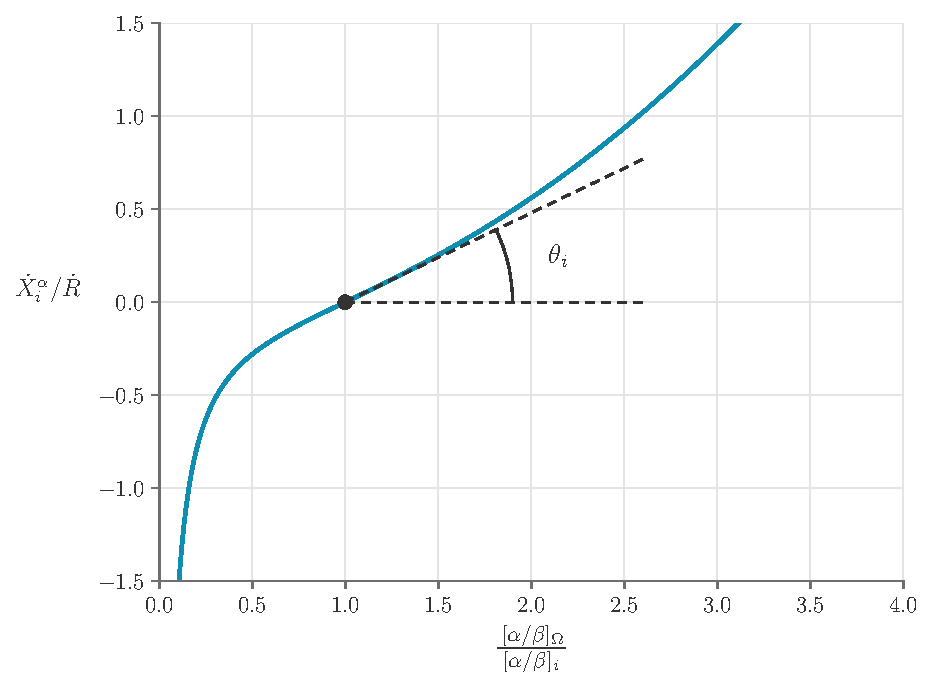
\includegraphics[width=0.75\textwidth]{degree_of_certainty.pdf}
    \caption{Geometrical interpretation of the participant's degree of certainty $\theta_i$}
    \label{figDegree}
\end{figure}
\clearpage

The same argument holds true if we want to plot a participant's exchange velocity using a logarithmic scale in $x$ (see Fig.~\ref{figDegreeLog}). In that case, the normalized axes are
\begin{equation*}
    x = \ln\!\left(\frac{\hspace{2pt}\priceAB_\Omega}{\priceAB_i}\right) \,\text{ and }\,
    y = \frac{\dot{X}_i^\alpha}{\dot{R}}\,,
\end{equation*}
and the expression for the exchange velocity becomes
\begin{equation*}
    y = w_i \left(\exp(2x) - \exp(-x)\right) \, .
\end{equation*}
Again, we find that
\begin{equation*}
    \tan \left( \theta_i \right) = \left.\frac{dy}{dx}\right|_{y=0} = 3\, w_i \,,
\end{equation*}
which leads to the relation between $\theta_i$ and $w_i$ that we were looking for
\begin{equation*}
    w_i = \frac{1}{3}\tan \left(\theta_i\right)\,.
\end{equation*}

Let us note that the last expression assumes that the angle $\theta_i$ is in radians and contained between 0 and $\pi/2$. To get the expression \eqref{eqFunctionW}, we linearly map $[0,\pi/2)$ to $[0,100)\%$. This leads to
\begin{equation*}
    w_i = \frac{1}{3}\tan \left(\frac{\pi\, \theta_i}{200\%}\right)\,,
\end{equation*}
in which $\theta_i$ is the participant's ``degree of certainty" contained between 0\% and 100\%.

\begin{figure}[b!]
    \centering
    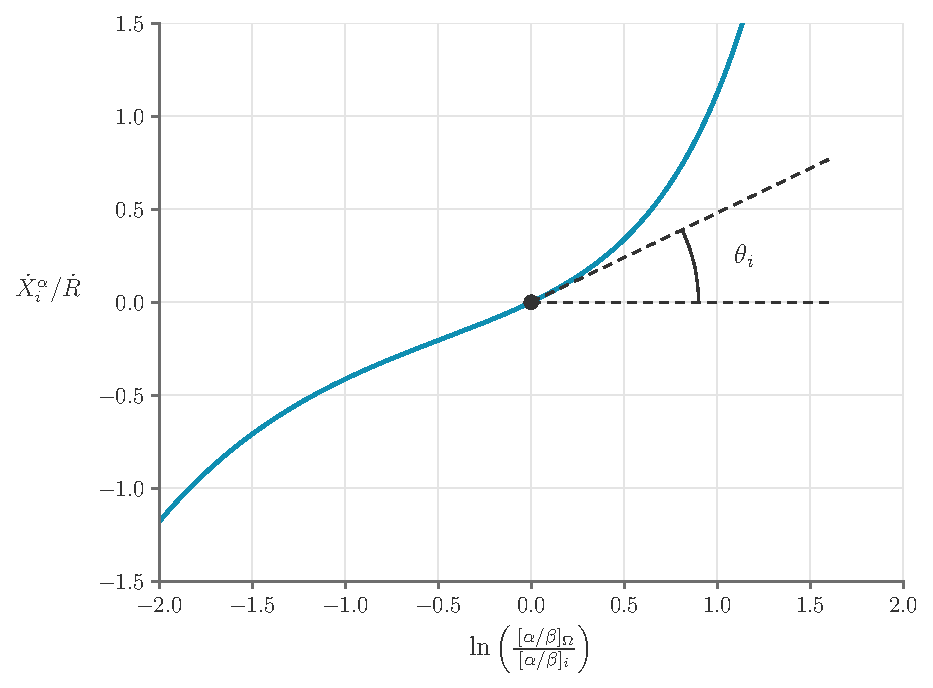
\includegraphics[width=0.75\textwidth]{degree_of_certainty_log.pdf}
    \caption{Geometrical interpretation of the participant's degree of certainty $\theta_i$}
    \label{figDegreeLog}
\end{figure}
\clearpage

\subsection{Proof that the exchange velocities function implies an exchange at market price}\label{secProofExchangeAtMarketPrice}
% ----------------------------------------------------------------------

We want to show that the expressions for a participant's exchange velocities defined in \eqref{eqExchangeVelocities} automatically satisfy the principle \eqref{eqExchangeAtMarketPrice}.

By constructing the right side of \eqref{eqExchangeAtMarketPrice}, using the expressions in \eqref{eqExchangeVelocities}, we get
\begin{align*}
    -\frac{\dot{X}^\alpha_i}{\dot{X}^\beta_i} &= -\frac{\hspace{-29pt}w_i \left( \left( \frac{\hspace{2pt}\priceAB_\Omega}{\priceAB_i}\right)^2 - \frac{\priceAB_i}{\hspace{2pt}\priceAB_\Omega} \right) \dot{R}}{w_i \left( \left( \frac{\hspace{2pt}\priceBA_\Omega}{\priceBA_i}\right)^2 - \frac{\priceBA_i}{\hspace{2pt}\priceBA_\Omega} \right) \dot{R} \priceBA_i}\\
    &= \frac{\hspace{12pt}\frac{\priceAB_i}{\hspace{2pt}\priceAB_\Omega} - \left( \frac{\hspace{2pt}\priceAB_\Omega}{\priceAB_i}\right)^2 }{\left( \frac{\hspace{2pt}\priceBA_\Omega}{\priceBA_i}\right)^2 - \frac{\priceBA_i}{\hspace{2pt}\priceBA_\Omega}} \priceAB_i\\
    &=\frac{\frac{\priceAB_i^3-\priceAB_\Omega^3}{\priceAB_\Omega \priceAB_i^2}}{\frac{\priceBA_\Omega^3-\priceBA_i^3}{\priceBA_i^2 \priceBA_\Omega}} \priceAB_i\\
    &= \left(\frac{\priceAB_i^3-\priceAB_\Omega^3}{\priceBA_\Omega^3-\priceBA_i^3} \right)\left(\frac{\priceBA_i^2 \priceBA_\Omega}{\priceAB_\Omega \priceAB_i^2} \right)\priceAB_i\\
    &= \left(\frac{\priceAB_i^3-\priceAB_\Omega^3}{\priceBA_\Omega^3-\priceBA_i^3} \right) \left(\priceBA_i^3 \priceBA_\Omega^3\right)\priceAB_\Omega\\
    &= \left( \frac{\priceBA_\Omega^3 - \priceBA_i^3}{\priceBA_\Omega^3 - \priceBA_i^3}\right) \priceAB_\Omega \\
    &= \priceAB_\Omega \,.
\end{align*}
\begin{flushright}
Q.E.D.
\end{flushright}

\subsection{The family of admissible trader functions}\label{secTraderFamily}
% ----------------------------------------------------------------------

The \tokEx{} defines its trader function as $f(x) = x^2 - 1/x$. This annex makes precise which part of that choice is forced by the principles and which part is a design decision, and it discloses the whole family of admissible alternatives.

\textbf{What the principles force.} Let $f$ be any candidate trader function, used symmetrically by both assets as in \eqref{eqExchangeSymmetry}, and write $x = \priceAB_\Omega / \priceAB_i$. The two velocities of the $i$\textsuperscript{th} participant are then $\dot{X}^\alpha_i = w_i f(x)\, \dot{R}$ and $\dot{X}^\beta_i = w_i f(1/x)\, \dot{R} \priceBA_i$. Principle 2 requires $-\dot{X}^\alpha_i / \dot{X}^\beta_i = \priceAB_\Omega = x \priceAB_i$ for every market state, which simplifies to the functional equation
\begin{equation}
    f(1/x) = -\frac{f(x)}{x} \qquad \text{for all } x > 0\,. \label{eqFunctionalEquation}
\end{equation}
At $x = 1$, \eqref{eqFunctionalEquation} gives $f(1) = -f(1)$, hence $f(1) = 0$: not trading at one's own estimate is not an extra hypothesis, it is a consequence of exchanging two symmetric assets at a single market price. The equation also determines $f$ on $(0,1)$ from its values on $(1,\infty)$: the selling behavior is the reflection of the buying behavior. Concretely, in absolute value, a participant facing a market at twice their estimate behaves exactly as one facing half of it, with the roles of the two assets exchanged (each velocity counted in the reference unit of its own asset); this mirror symmetry is shared by every admissible trader function, and is the one visible in Fig.~\ref{figExchangeSymmetry}.

\textbf{The closed-form family.} Consider the power pairs
\begin{equation}
    f_p(x) = x^p - x^q\,, \qquad q = 1 - p\,, \quad p \geq 1\,. \label{eqTraderFamily}
\end{equation}
Every member satisfies \eqref{eqFunctionalEquation}, since $q - 1 = -p$ and $p - 1 = -q$. For $p \geq 1$ the member is strictly increasing on $(0, \infty)$, with $f_p'(x) = p\,x^{p-1} + (p-1)\,x^{-p} > 0$, and therefore satisfies principles 5 to 8 (for $1/2 < p < 1$ monotonicity fails near $0$, and $p = 1/2$ gives the zero function). Replacing $f$ by $f_p$ in \eqref{eqExchangeSymmetry} and solving the equilibrium condition \eqref{eqEquilibrium} yields the market price in closed form,
\begin{equation}
    \priceAB_\Omega = \left( \frac{\displaystyle \sum_i w_i \priceAB_i^{\,p-1}}{\displaystyle \sum_i w_i \priceBA_i^{\,p}} \right)^{1/(2p-1)}\,, \label{eqFamilyPrice}
\end{equation}
and the slope at the equilibrium point is $f_p'(1) = 2p - 1$, so that the degree-of-certainty map of the member reads $w = \frac{1}{2p-1} \tan\left(\pi\,\theta/200\,\%\right)$. All the results of this document (uniqueness of the price, aggregation of the market into a single participant, the two algorithms) carry over member by member. More generally, any combination $\sum_p c_p f_p$ with nonnegative coefficients satisfies \eqref{eqFunctionalEquation} and the principles, though the closed form \eqref{eqFamilyPrice} is then lost.

\textbf{What singles out $p = 2$.} The first member, $f_1(x) = x - 1$, has a bounded selling side: $f_1(x) > -1$ for all $x > 0$, so a participant's urgency would saturate at $w_i \dot{R}$ no matter how far the market price drops below their estimate. For every $p > 1$, both sides are unbounded: $f_p \to +\infty$ as $x \to \infty$ and $f_p \to -\infty$ as $x \to 0^+$. Among the members with integer exponents (Laurent polynomials), the smallest one with unbounded urgency on both sides is therefore $p = 2$:
\begin{equation*}
    f_2(x) = x^2 - \frac{1}{x}\,,
\end{equation*}
the trader function \eqref{eqTraderFunction} of the \tokEx{}, whose slope $2p - 1 = 3$ is the factor of \eqref{eqFunctionW}.

\textbf{Disclosure.} The whole family \eqref{eqTraderFamily}, together with the corresponding market price \eqref{eqFamilyPrice} and degree-of-certainty map, is part of the present disclosure: an exchange mechanism obtained by substituting any member $f_p$ (or any nonnegative combination of members) for the trader function of the \tokEx{} is anticipated by this document.

\subsection{Proof that the expression for the market price corresponds to the equilibrium between supply and demand}\label{secProofMarketprice}
% ----------------------------------------------------------------------

By making the hypothesis that~\eqref{eqEquilibrium} holds for asset A and by applying principle number 2, stating that the market price is the same for every participant at any given time and that the market price is strictly positive, we can derive expression \eqref{eqMarketPrice} as such:
\begin{align*}
    0 &= \sum_i \dot{X}_i^\alpha\\
    0 &= \sum_i w_i \left( \left( \frac{\hspace{2pt}\priceAB_\Omega}{\priceAB_i}\right)^2 - \frac{\priceAB_i}{\hspace{2pt}\priceAB_\Omega} \right) \dot{R} \\
    0 &= \sum_i w_i \left( \priceBA_i^2 - \priceBA_\Omega^3 \priceAB_i \right) \priceAB_\Omega^2 \dot{R}\\
    0 &= \sum_i w_i \priceBA_i^2 - \priceBA_\Omega^3 \sum_i w_i \priceAB_i\\
    \priceAB_\Omega &= \left( \frac{\displaystyle \sum_i w_i \priceAB_i}{\displaystyle \sum_i w_i \priceBA_i^2}\right)^{1/3} \,.
\end{align*}
\begin{flushright}
Q.E.D.
\end{flushright}
Since we have already proven that
\begin{equation*}
    \sum_i \dot{X}_i^\alpha = 0 \text{ and that }\priceAB_\Omega = -\frac{\dot{X}_i^\alpha}{\dot{X}_i^\beta}\,,
\end{equation*}
we can quickly show that the exchanges of asset~B also satisfy \eqref{eqEquilibrium} in the following manner
\begin{align*}
    \sum_i \dot{X}_i^\beta &= -\priceBA_\Omega \sum_i \dot{X}_i^\alpha\\
    \sum_i \dot{X}_i^\beta &= 0 \,.
\end{align*}
\begin{flushright}
Q.E.D.
\end{flushright}

\subsection{Proof that the market price is unique}\label{secProofUniqueness}
% ----------------------------------------------------------------------

Annex~\ref{secProofMarketprice} is conditional: it shows that \emph{if} an equilibrium price exists, it must be \eqref{eqMarketPrice}. This annex closes the argument by showing that exactly one equilibrium price always exists, so that the market price of principle 1 is well defined and the inner algorithm is deterministic.

\textbf{Conditions.} Every estimate is strictly positive, every weight is nonnegative, and at least one trading participant carries a strictly positive weight:
\begin{equation*}
    \priceAB_i > 0 \ \text{ for all } i\,, \qquad w_i \geq 0 \ \text{ for all } i\,, \qquad \exists\, j: w_j > 0\,.
\end{equation*}

\textbf{Claim.} Under these conditions, there is exactly one strictly positive price at which the market is in equilibrium, and it is the one given by \eqref{eqMarketPrice}.

\textbf{Proof.} Consider the net flow of asset A as a function of a candidate price $z > 0$:
\begin{equation*}
    g(z) = \sum_i w_i \left( \left(\frac{z}{\priceAB_i}\right)^2 - \frac{\priceAB_i}{z} \right) \dot{R}\,.
\end{equation*}
Each term with $w_i > 0$ is strictly increasing in $z$, since
\begin{equation*}
    \frac{d}{dz}\left[ w_i \left( \left(\frac{z}{\priceAB_i}\right)^2 - \frac{\priceAB_i}{z} \right) \right] = w_i \left( \frac{2z}{\priceAB_i^2} + \frac{\priceAB_i}{z^2} \right) > 0\,,
\end{equation*}
and each term with $w_i = 0$ vanishes identically. As at least one weight is strictly positive, $g$ is strictly increasing on $(0, \infty)$. Moreover, $g(z) \to -\infty$ as $z \to 0^+$ (the $-\priceAB_i/z$ terms dominate) and $g(z) \to +\infty$ as $z \to \infty$ (the quadratic terms dominate). Since $g$ is continuous and strictly increasing with these limits, it vanishes at exactly one $z > 0$. By Annex~\ref{secProofMarketprice}, that zero is \eqref{eqMarketPrice}.
\begin{flushright}
Q.E.D.
\end{flushright}

\textbf{Corollary.} Every term of $g$ is nonpositive at $z = \min_i \priceAB_i$ (all ratios $z/\priceAB_i \leq 1$) and nonnegative at $z = \max_i \priceAB_i$; the equilibrium price therefore always lies between the smallest and the largest estimate of the trading participants.

\subsection{Proof that the total market behaves as a single participant}\label{secProofTotalMarketWeight}
% ----------------------------------------------------------------------

In \eqref{eqDefMarketBehavior}, we defined the market behavior as the sum of the behavior of all its participants
\begin{equation*}
    \dot{X}_\Omega^\alpha = \sum_i w_i \left( \left( \frac{\priceAB_z}{\priceAB_i}\right)^2 - \frac{\priceAB_i}{\priceAB_z} \right) \dot{R} \,.
\end{equation*}
We want to prove that there exists a total market weight $W_\Omega$ such that the market behaves as a single participant, in a way that
\begin{equation*}
    W_\Omega\left(\left(\frac{\priceAB_z}{\priceAB_\Omega}\right)^2-\frac{\priceAB_\Omega}{\priceAB_z}\right) \dot{R} = \sum_i w_i \left( \left( \frac{\priceAB_z}{\priceAB_i}\right)^2 - \frac{\priceAB_i}{\priceAB_z} \right) \dot{R} \,,
\end{equation*}
for any $\priceAB_z$.

Of course, this statement is true in the trivial case when the inputs of each of the $N_\Omega$ participants are $\priceAB_i = \priceAB_\Omega$ and $w_i=W_\Omega / N_\Omega$, but we want to prove that it is in fact true for any participant's inputs.

By looking at the previous expression term by term, we conclude that for it to be true for any $\priceAB_z$, we must satisfy both
\begin{align*}
    W_\Omega \priceBA_\Omega^2 &= \sum_i w_i \priceBA_i^2 \, \text{ and}\\
    W_\Omega \priceAB_\Omega &= \sum_i w_i \priceAB_i\,.
\end{align*}
We can easily satisfy the second expression by setting
\begin{equation*}
    W_\Omega = \priceBA_\Omega \sum_i w_i \priceAB_i\,.
\end{equation*}

Now, we need to verify that this choice also satisfies the first expression
\begin{align*}
    W_\Omega \priceBA_\Omega^2 &= \sum_i w_i \priceBA_i^2 \\
    \left(\priceBA_\Omega \sum_i w_i \priceAB_i\right) \priceBA_\Omega^2 &= \sum_i w_i \priceBA_i^2\\
    \priceBA_\Omega^3 \sum_i w_i \priceAB_i &= \sum_i w_i \priceBA_i^2\\
    \priceAB_\Omega &= \left(\frac{\displaystyle \sum_i w_i \priceAB_i}{\displaystyle \sum_i w_i \priceBA_i^2} \right)^{1/3} \,.
\end{align*}
The last line corresponds to the expression for the market price that we already proved in Annex~\ref{secProofMarketprice}.

\begin{flushright}
Q.E.D.
\end{flushright}

\subsection{Statistical interpretation of the equation for the total market weight}\label{secStatisticalInterpretation}
% ----------------------------------------------------------------------

The equation defining the total market weight can be rearranged as
\begin{equation*}
    \priceAB_\Omega = \sum_i \frac{w_i}{W_\Omega} \priceAB_i\,.
\end{equation*}

Since the market price $\priceAB_\Omega$ is in some sense the weighted average of the participants' estimates $\priceAB_i$, one can draw a parallel between the previous expression and the expected value of a random variable $X$, which is by definition
\begin{equation*}
    E[X] = \sum_i p_i \,x_i \,
\end{equation*}
where $x_i$ is a particular outcome of the variable $X$ and $p_i$ is the probability of getting this particular outcome.

In this analogy, we have that:
\begin{align*}
    X &\rightarrow \priceAB \, ,\\
    E[X] &\rightarrow \priceAB_\Omega \, , \\
    p_i &\rightarrow \frac{w_i}{W_\Omega} \, ,\\
    x_i &\rightarrow \priceAB_i \,.
\end{align*}

Now if $\priceAB_\Omega$ is the expected value of the random variable $\priceAB$, then we may ask what is its variance. The variance of a random variable can be calculated using
\begin{equation*}
    \mathrm{Var}(X) = E[X^2] - (E[X])^2 \, .
\end{equation*}

Thus, we find that the quantity analogous to the variance of the participants' estimates is
\begin{equation*}
    \mathrm{Var}(X) \rightarrow \frac{1}{W_\Omega} \sum_i w_i \priceAB_i^2 - \priceAB_\Omega^2  \, .
\end{equation*}

\end{document}
